\documentclass[conference]{IEEEtran}
\IEEEoverridecommandlockouts
% The preceding line is only needed to identify funding in the first footnote. If that is unneeded, please comment it out.
\usepackage{cite}
\usepackage{amsmath,amssymb,amsfonts}
\usepackage{algorithmic}
\usepackage{graphicx}
\usepackage{textcomp}
\usepackage{xcolor}
\usepackage{color, colortbl}

\bibliographystyle{IEEEtran}

\begin{document}

\title{Using self-supervised learning to decrease the need for labeled data in medical image object detection\\
\thanks{This work was supported in part by the Croatian Science Foundation under Project UIP-2017-05-4968.}
}

\author{\IEEEauthorblockN{Marin Benčević\IEEEauthorrefmark{1}\IEEEauthorrefmark{2}, Marija Habijan\IEEEauthorrefmark{1}, Irena Galić\IEEEauthorrefmark{1}, Aleksandra Pizurica\IEEEauthorrefmark{3}} 
\IEEEauthorblockA{\IEEEauthorrefmark{1}Faculty of Electrical Engineering, Computer Science and Information Technology\\
J. J. Strossmayer University of Osijek, Osijek, Croatia}
\IEEEauthorblockA{\IEEEauthorrefmark{2}Email: marin.bencevic@ferit.hr} 
\IEEEauthorblockA{\IEEEauthorrefmark{3}TELIN-GAIM, Faculty of Engineering and Architecture\\
Ghent University, Ghent, Belgium}}

\maketitle

\begin{abstract}
This document is a model and instructions for \LaTeX.
This and the IEEEtran.cls file define the components of your paper [title, text, heads, etc.]. *CRITICAL: Do Not Use Symbols, Special Characters, Footnotes, 
or Math in Paper Title or Abstract.
\end{abstract}

\begin{IEEEkeywords}
component, formatting, style, styling, insert
\end{IEEEkeywords}



\section{Introduction}

One of the largest problems in medical image processing is the lack of annotated data. To function 
robustly and to show their generalizability potential, deep learning networks require a large 
amount of annotated images \cite{litjensSurveyDeepLearning2017}. However, 
annotating medical imaging is often time-consuming, precise work. There is a need to improve the 
data efficiency and robustness of deep learning networks for medical image processing
trained on smaller datasets. Furthermore, 
there is a need to make the labeling process faster to save experts' time. This paper presents a 
step towards both of those goals. The primary contribution of this paper is the evaluation a method 
which uses self-supervised learning 
to extract salient information from \textit{unlabeled} images which can then be used to more 
easily train a object detection deep learning network on a more limited dataset 
of \textit{labeled} images.

Improving data efficiency in medical object detection is of particular importance. 
In terms of labeling complexity, it is 
simpler and quicker to label a dataset with bounding boxes than to label each instance as is 
needed for semantic segmentation. In a lot of medical imaging tasks, a precise semantic 
segmentation map is not required, and a bounding box communicates sufficient information for 
further diagnosis, treatment or research on a given image. By improving data efficiency for 
bounding box labels, we hope to increase their usefulness and thus save time by allowing experts 
to use bounding box labels in place of semantic segmentation maps for some medical image processing
tasks.

In this paper, we show that it is possible to improve the performance of an object detection model
for medical images by utilizing self-supervised learning in a pretraining phase. In addition, we
also show that it is possible to achieve similar performance to a fully supervised model with
only 60\% of the labeled data by utilizing self-supervised pretraining.

\subsection{Related work}

There are several ways to try to utilize unlabeled data or data prepared for other tasks to improve
the data efficiency of medical image processing. The most common approach in medical image tasks is
to use transfer learning on large image datasets 
such as ImageNet, however Raghu et al. \cite{raghuTransfusionUnderstandingTransfer2019} found that
this provides little benefit in medical image processing tasks in terms of performance, but does
improve convergence speed during training.

Some works use semi-supervised learning to utilize an unlabeled dataset to improve
performance of a model. These approaches generally work by utilizing statistical features
of an unlabeled dataset while simultaneously training on a labeled dataset. The unlabeled
dataset is mined for soft signals to nudge the model towards better overall performance.
One such example is the one by Liu et al. \cite{liuSemisupervisedMedicalImage2020} where
they present a semi-supervised learning method for medical image classification using
a combination of unlabeled and labeled data from the same domain.

TODO OBJECT DETECTION HINDAWI PAPER.

\subsubsection{Self-supervised learning}

Recently more and more papers use self-supervised learning to pre-train neural networks on
unlabeled data, and then fine tune the networks on the available labeled data.
Self-supervised learning is a method of unsupervised neural network training where a
an encoder is trained to learn salient features or embeddings of an input. The
goal is to train an encoder which will understand useful features for a downstream
task such as object detection, classification or similar. Self-supervised learning has
been shown to improve data efficiency
\cite{chenSimpleFrameworkContrastive2020} as well as robustness to dataset imbalance
\cite{liuSelfsupervisedLearningMore2021}.

There are several approaches of training the encoder such that it learns useful features.
One approach is to use a constructed task which uses the unlabeled data and for which one
can automatically obtain the correct solution, so that the correct solution can be used
for supervised training. An example of this approach is presented by Noroozi and Favaro 
\cite{norooziUnsupervisedLearningVisual2016} where the neural network is trained to 
solve a jigsaw constructed from an unlabeled dataset.

Recently, a more common approach to self-supervised pretraining is contrastive learning.
In contrastive learning, the encoder is trained to minimize the distance between feature
vectors of positive examples, and maximize the distance between negative examples. The
positive examples are constructed in an unsupervised manner by e.g. randomly augmenting
and image twice, thus producing two examples for which the feature vectors should be
similar. Among others, notable examples of such approaches are SimCLR 
\cite{chenSimpleFrameworkContrastive2020} and MoCo \cite{he2019moco}.

\subsubsection{Self-supervised learning in medical images}

There are a number of papers both the constructed task approach 
(\cite{baiSelfSupervisedLearningCardiac2019}, \cite{ZHU2020101746}) as well as contrastive
learning (\cite{zhouComparingLearnSurpassing2020}). There are also a number of papers
that evaluate self-supervised pretraining on an unlabeled subset of the data for medical
imaging tasks. Taleb et al. \cite{NEURIPS2020_d2dc6368} evaluate a variety of 
self-supervised pretraining approaches
for medical image segmentation in 3D MRI and CT images as well as classification on 2D 
fundus photograpy images. They use unlabeled data of the same modality but from a 
different corpus. Azizi et al. \cite{aziziBigSelfSupervisedModels2021} introduce a
novel contrastive learning method and evaluate it at various percentages of used
dataset labels on dermatology and chest X-ray classification. However, to the
best of our knowledge the are currently no papers which evaluate self-supervised 
pretraining for object detection tasks in medical images.



\section{Dataset description and demographics}\label{dataset}

The dataset used in this paper is a dataset of 15,000 labeled chest radiographs called VinDr-CXR, 
described in more detail in \cite{nguyenVinDrCXROpenDataset2021}. While the original dataset 
contains 3,000 additional test images, we were not able to obtain the labels for these images, and 
they were not used in this paper. Each scan of the dataset was labeled by three separate 
radiologists.  The dataset was collected from two major Vietnamese hospitals. 

We chose this dataset as a good indicator of the generalizability of the findings in this paper 
due to several reasons. Firstly, to our knowledge, this is the largest radiograph dataset with 
bounding box labels for each finding. Secondly, having multiple labels for each image allows us to 
perform a large variety of statistical evaluation methods, such as comparing the inter-observer 
variability. Having multiple labels also allows us to use automatic methods to find a concensus 
between them, possibly leading to less noisy annotations.

\subsection{Data preparation}

Each DICOM image from the dataset was resized to a resolution of 512 $\times$ 512 pixels. We 
discard all examples for which there is no anomaly found (examples labeled as "no finding"). After 
discarding, we are left with a total of 4,394 images. We randomly split this dataset into a 
training set (70\%, 3075 images), validation set (10\%, 440 images) and a test set (20\%, 878 
images). The training set was used to train the models, the validation set was used to tune the 
model hyperparameters and determine when to stop training, and the test set is used for final 
evaluation. The model did not have access to the test set during training.

The original dataset differentiates 14 different classes, one of which is the "no finding" class. 
We discard this class, resulting in 13 possible class labels. The class distribution of the full 
dataset is shown in Fig. \ref{fig:class-balance}.

Each image can have one or more 
labels from multiple experts, and these labels often overlap. To produce the least noisy labels, 
we fused overlapping labels from multiple experts into one label by finding an average rectangle 
of several overlapping rectanges. To determine if two rectangles are overlapping, an intersection-over-union 
(IoU) threshold of 20\% is used. A rectangle ${R_i}$ is defined by its top-left corner 
$(X_{i1}, Y_{i1})$ and its bottom-right corner $(X_{i2}, Y_{i2})$. An average rectangle $\bar{R}$ 
defined by coordinates $(\bar{X_{1}}, \bar{Y_{1}})$ and $(\bar{X_{2}}, \bar{Y_{2}})$ where each 
coordinate is an average of the appropriate coordinates in all of the rectangles to be averaged.
This approach is based on weighted boxes fusion 
described in \cite{solovyevWeightedBoxesFusion2021}, but modified such that each bounding box has 
equal weight and confidence since they were manually labeled by an expert. An example of fused 
bounding boxes is shown in Fig. \ref{fig:wbf}.

\begin{figure}[h]
\centering
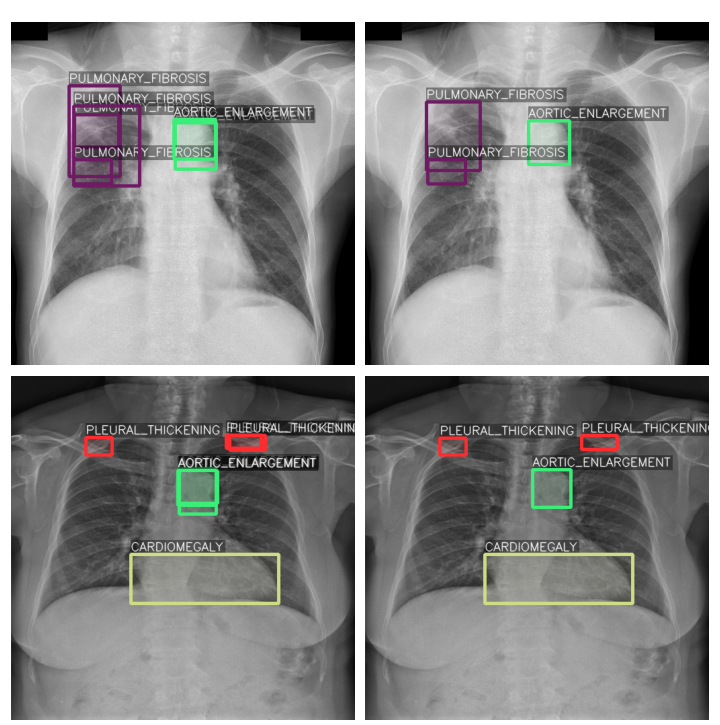
\includegraphics[width=\columnwidth]{images/wbf}
\caption{Examples of bounding box averaging. The images on the left show the original bounding boxes, while the images on the right show fused bounding boxes which are used in our experiments.}
\label{fig:wbf}
\end{figure}

% TODO Figure wbf

\section{Methods}

The main goal of this paper is to analyze gow self-supervised model pre-training affects data efficiency for object detection in medical images. Therefore, we first train a baseline deep learning model with no pre-traning and on the full labeled traning dataset following a standard approach for this type of problem. This model will be used as a point of comparison to more objectively evaluate the pre-trained models.

To evaluate the pre-training, we randomly split the traning dataset into two separate datasets, a pre-traning and fine-tuning dataset. For the pre-traning dataset we discard all class labels, as this dataset will be used to pre-train the model using self-supervised learning on unlabeled data. The fine-tuning dataset will then be used to fine-tune the pre-trained model using standard supervised learning. We train nine different pre-trained models in total, ranging from 10\% to 90\% of the total training set in the unlabeled pre-train dataset, in increments of 10\%. A summary of our approach is shown in \ref{fig:dataset-split-summary}.

\begin{figure}[h]
\centering
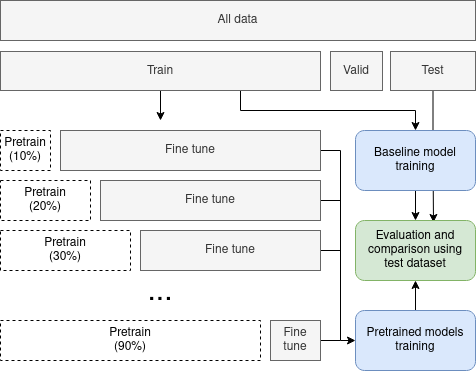
\includegraphics[width=\columnwidth]{images/dataset-split-summary}
\caption{A summary of our experiments. A percentage of the training dataset is moved to the pre-training dataset and models are pre-trained using the pre-training datasets and then fine tuned with the rest of the training data. The pre-training datasets are unlabeled. A separate baseline model is trained using the full labeled dataset.}
\label{fig:dataset-split-summary}
\end{figure}

\subsection{Balancing the dataset}

As shown in Figure \ref{fig:class-balance} the dataset is highly imbalanced. To improve class-balance during training we oversample examples with less-represented classes. We use the oversampling approach described in \cite{gupta2019lvis}. The general approach is as follows:

\begin{enumerate}
\item For each class $c$, compute it's frequency $f(c)$ in the training set.
\item Compute a class repeat factor $r(c) = max(1, \sqrt{{t}/{f(c)}})$, where $t$ is a threshold value empericially set to 0.4 in our experiments. The value of 0.4 produced the maximum validation mean average precision for the baseline model.
\item For each image $I$, compute an image repeat factor $r(I) = C * r(c)$ where $C = max(r(c_i))$ for each class $c_i$ in image $I$.
\end{enumerate}

This balancing is performed on-line during training and only on the training set. We found that balancing the dataset in this way significantly improved the mean average precision when averaged across all classes.

\begin{figure}[h]
\centering
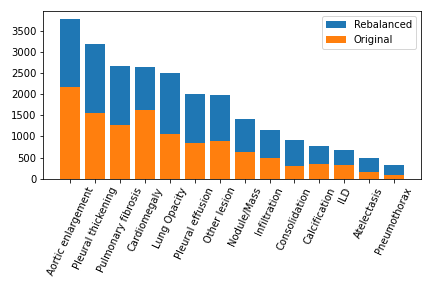
\includegraphics[width=\columnwidth]{images/rebalace}
\caption{A histogram of the class balance of the original dataset (by number of images containing the class), and the same histogram for our oversampled dataset.}
\label{fig:class-balance}
\end{figure}

\subsection{Baseline model details}

For an objective and fair comparison, we train a baseline model using a standard deep learning-based approach for object detection. We use a Faster R-CNN-based model \cite{DBLP:conf/nips/RenHGS15} with a ResNet50 encoder \cite{He_2016_CVPR}. The model is initialized using pre-trained weights trained on the COCO dataset for 12 epochs, a batch size of 2 and using the SGD optimizer with a learning rate of 0.0002, momentum of 0.9 and a weight decay of 0.0001.

\subsection{Pretraining model details}

The pretraining model we use is a SimCLR-based model \cite{chenSimpleFrameworkContrastive2020} to pre-train a ResNet-50 backbone, the same backbone used in the baseline model. We train the SimCLR model (described later in this section) using the unlabeled pre-training dataset. We then use the pre-trained backbone in the same model as our baseline model and fine-tune the final model on the fine-tuning dataset. The result is a model similar to our backbone model but trained on fewer labeled data.

SimCLR uses contrastive learning where an example image is augmented randomly twice and each augmentation is fed into a separate encoder branch, where the branches use shared weights. The network outputs two feature maps, one for each augmentation. The loss function measures the difference between these two feature maps. The closer the two feature maps are, the lower the loss. This ensures that two augmentations from the same example will produce similar feature maps, thus making the network learn salient features which are invariant to the chosen augmentations.

In our experiments, we use the following augmentations for SimCLR training:

\begin{enumerate}
\item A random crop and resize of the original image by a factor of 0.2 to 1.
\item A random horizontal flip (with a 50\% chance).
\item A random Gaussian blur with $\sigma$ between 0.1 and and 2, and a kernel size of 21.
\item A random amount of Gaussian noise with $\sigma$ being a random number between 12.5\% and 25\% of the mean image pixel value.
\end{enumerate}

In addition, each training and validation image has histogram normalization applied.

\section{Results}\label{sec2}

A summary of the results of our experiments is shown on Table \ref{tab:results}. All of the results in this section are calculated on the testing dataset. Our main evaluation metrics are the mean average precision (mAP), averaged across all classes and IoU thresholds from 0.5 to 0.95 in 0.05 intervals (mAP@[.5, .95]), as is standard for benchmarking the COCO dataset. We also calculate the mAP at a fixed IoU of 0.5 (mAP@0.5), which is standard for evaluating models on the PASCAL VOC dataset. These metrics are also calculated class-wise. In addition, we calculate the average recall given 100 detections per image (AR@100).

\definecolor{LightGray}{gray}{0.9}

\begin{table}[h]
\renewcommand{\arraystretch}{1.3}
% TODO: Cite COCO and PASCAL VOC?
\caption{A summary of the results of our experiments. mAP is the mean average precision at IoU values from 0.5 tp 0.95 at 0.05 (mAP@[.5, .95]) increments across all classes, the standard metric for the COCO benchmark. mAP50 is the mAP at IoU = 50\% (mAP@0.5), the standard metric for the PASCAL VOC benchmark. mAP small is the mAP@[.5, .95] for objects with an area smaller than 32 pixels$^2$. AR is the average recall given 100 detections per image (AR@100). AR small is the same as AR but only for objects with an area smaller than 32 pixels$^2$. Training images is the total number of labeled training examples available to the model.}
\label{tab:results}
\centering
\begin{tabular}{|c|c|c|c|c|c|c|c}
\hline
\begin{minipage}{5mm} ~\\ \\ \\ \end{minipage} & mAP & mAP50 & \parbox[c]{7mm}{mAP\\small} & AR & \parbox[c]{7mm}{AR\\small} & \parbox[c]{9mm}{Training\\images} \\ \hline \hline
\rowcolor{LightGray}
Baseline & 0.129 & 0.278 & 0.021 & 0.412 & 0.154 & 3075 \\ \hline
SSL 10\% & \textbf{0.142} & 0.284 & \textbf{0.026} & \textbf{0.413} & 0.156 & 2767 \\ \hline
SSL 20\% & 0.139 & \textbf{0.292} & 0.020 & 0.412 & \textbf{0.158} & 2460 \\ \hline
SSL 30\% & 0.130 & 0.268 & 0.014 & 0.402 & 0.146 & 2152 \\ \hline
SSL 40\% & 0.123 & 0.272 & 0.014 & 0.394 & 0.131 & 1845 \\ \hline
\rowcolor{LightGray}
SSL 50\% & 0.109 & 0.248 & 0.011 & 0.387 & 0.131 & 1537 \\ \hline
SSL 60\% & 0.104 & 0.230 & 0.011 & 0.378 & 0.120 & 1230 \\ \hline
SSL 70\% & 0.095 & 0.202 & 0.007 & 0.363 & 0.108 & 922 \\ \hline
SSL 80\% & 0.081 & 0.178 & 0.006 & 0.338 & 0.089 & 615 \\ \hline
SSL 90\% & 0.060 & 0.135 & 0.003 & 0.303 & 0.064 & 307 \\
\hline
\end{tabular}
\end{table}

The baseline model, trained on all of the labeled data, achieves an mAP of 0.129. By adding pretraining on 10\% of the data (i.e. removing 10\% of the labels) the mAP increases to 0.142. This is the best-performing model in our experiments. In addition, by additing pretraining on a small percentage of the dataset (20\% or fewer) the performance improves for all of the metrics we calculated. However, even with just 60\% of the labeled data we achieve an mAP of 0.123, only slightly smaller than the baseline model. In terms of percentages, with only 60\% of the labels we still achieve more than 95\% of the performance of the baseline model in terms of mAP. Similar results can be see in terms of recall — the baseline model achieves an AR of 0.412 while with 60\% of the labels we achieve an AR of 0.394, more than 95\% of the base model's AR.

However, the differences are larger when looking at small objects. While the baseline model achieves a 0.021 mAP for small objects, the model trained on 60\% of the labeled images achieves a small objects mAP of 0.014, 66.66\% of the baseline model. Similarly, the model trained on 60\% of the labeled images achieves a small object AR of 0.131, 85\% of the baseline model's small object AR of 0.154.

A graphical summary of the class-wise results is shown in Fig. \ref{fig:classwise-map}. The performance on most classes drops off linearly between the baseline model and the model trained on 60\% of the labels data. The dropoff becomes more significant after training on less than 60\% of the labels. In all cases the mAP at 60\% of the labeled data is highly correlated with the mAP across all classes as described earlier in the section, and the same conclusions apply to all classes.

\begin{figure}[h]
\centering
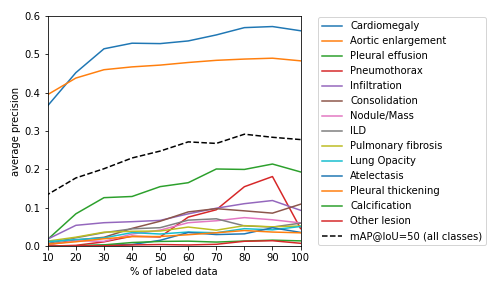
\includegraphics[width=\columnwidth]{images/map_graph}
\caption{The mean average precision (mAP@[.5, .95] across different percentages of labeled data for different classes in the dataset. The model at 100\% of labeled data is the baseline model.}
\label{fig:classwise-map}
\end{figure}

The model performs the best at detecting cardiomegaly and aortic enlargement, two classes with a large number of examples and large average object area size. All of the models perform significantly worse at detecting other anomalies. However, by adding pretraining on a small percentage of the data (20\% or fewer) the mAP improves for almost all classes, most significantly for detecting other lesions and infiltration.

TODO INTER-OBSERVER VARIABILITY, MAP60 COMPARISON WITH HINDAWI PAPER

\section{Discussion}\label{sec12}

Discussions should be brief and focused. In some disciplines use of Discussion or `Conclusion' is interchangeable. It is not mandatory to use both. Some journals prefer a section `Results and Discussion' followed by a section `Conclusion'. Please refer to Journal-level guidance for any specific requirements. 

\section{Conclusion}\label{sec13}

Conclusions may be used to restate your hypothesis or research question, restate your major findings, explain the relevance and the added value of your work, highlight any limitations of your study, describe future directions for research and recommendations. 

In some disciplines use of Discussion or 'Conclusion' is interchangeable. It is not mandatory to use both. Please refer to Journal-level guidance for any specific requirements. 

\bibliography{bibfile.bib}

\end{document}
